\subsection{Boundary Conditions}
In this section we will determine the value of $\ell$ that we used before for our semi-infinite and slab solutions \cite{haskell_94_1}. We start by defining the radiance ($\rm{W/m^2sr^1}$), which measures the amount of light passes through a given area within some solid angle in a specific direction. Integrating the radiance over all possible angles will give us the fluence rate that we've been using thus far. 
\begin{eqnarray}
\Phi({\bf r}) &=& \int\int_{4\pi} d\Omega \ L({\bf r},{\bf s})\\
{\bf j}({\bf r}) &=& \int\int_{4\pi} d\Omega \ L({\bf r},{\bf s}) \ {\bf s}
\end{eqnarray}
In the diffusion approximation, the radiance can be approximated by an isotropic fluence rate term plus an additional term for some small directional flux pointing along ${\bf s}$:
\begin{equation}
\label{Radiance}
L({\bf r},{\bf s}) = \frac{1}{4\pi} [ \Phi({\bf r}) + 3 {\bf j}({\bf
  r}) \cdot {\bf s}] \ .
\end{equation}
\begin{figure}[h]
\centering
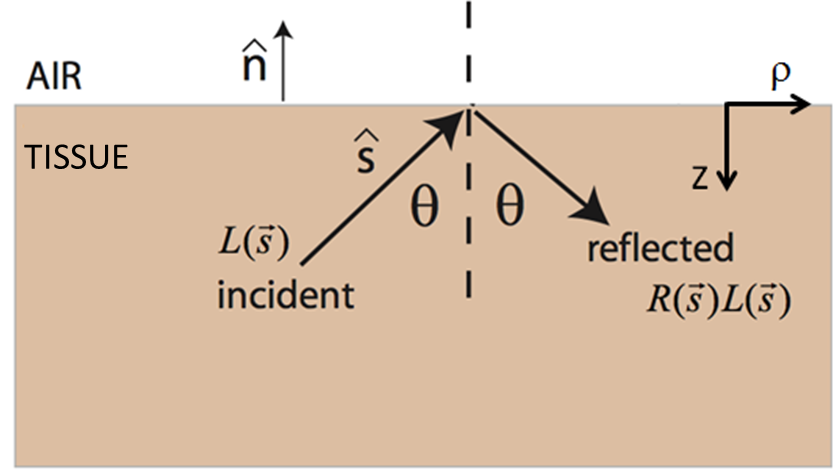
\includegraphics[width=8cm]{./figures/2_Theory/BoundaryReflect.png}
\caption{At the boundary, some of the incident light is Fresnel reflected back into the media due to index mismatch. This reflected light accounts for all of the light that is diffusing inwards towards the media at the boundary.}
\label{BoundaryReflect}
\end{figure}
Since we are interested in taking noninvasive measurements, we will look at the radiance at the air-tissue boundary. If ${\bf n}$ is the outward normal the tissue surface and ${\bf s}$ gives us the direction of the light propagation, then the fluence rate of the light exiting and entering the tissue is given by integrating $L({\bf s}) ({\bf s} \cdot {\bf n})$ over all outward directions and integrating  $L({\bf s}) ({\bf s} \cdot {- \bf n})$ over all inward directions
respectively. Air is not a scattering medium so there is no light entering the tissue from the boundary with the exception of the Fresnel reflected light of the outgoing light due to the index mismatch at the boundary. If $R({\bf \theta})$ is the Fresnel reflection coefficient for unpolarized light, then
\begin{equation}
\label{bc1}
\int\int_{{\bf s} \cdot {\bf n} > 0} R({\bf s}) L({\bf s}) ({\bf s} \cdot {\bf n}) d\Omega =
\int\int_{{\bf s} \cdot {\bf n} < 0} L({\bf s}) ({\bf s} \cdot {- \bf
  n}) d\Omega \ .
\end{equation}
\begin{equation}
\label{bc2}
\frac{1}{4\pi}\int\int_{{\bf s} \cdot {\bf n} > 0} R({\bf s}) [ \Phi({\bf r}) + 3 {\bf j}({\bf r}) \cdot {\bf s}] ({\bf s} \cdot {\bf n}) d\Omega = \frac{1}{4\pi} \int\int_{{\bf s} \cdot {\bf n} < 0} [ \Phi({\bf r}) + 3 {\bf j}({\bf r}) \cdot {\bf s}] ({\bf s} \cdot {-\bf n}) d\Omega \ .
\end{equation}
Changing into spherical coordinates, ${\bf s}\cdot{\bf n}=\cos\theta$ and ${\bf j}\cdot{\bf n}=j_z\cos\theta$, the integral
on the RHS then becomes
\begin{eqnarray}
\label{bc3}
\frac{1}{4\pi}\int\int_{{\bf s} \cdot {-\bf n}} [-\Phi\cos\theta + 3j_z\cos^2\theta]\sin\theta d \phi d\theta &=& \frac{1}{4}\int_{\pi/2}^{\pi} [-\Phi\cos\theta + 3j_z\cos^2\theta]\sin\theta d\theta \nonumber\\ 
&=&\frac{1}{2}\int_{0}^{-1} [\Phi u - 3j_zu^2] du \notag \\
&=&\frac{\Phi}{4}+\frac{j_z}{2}
\end{eqnarray}
\noindent
where I have used $u=\cos\theta$ substitution to get the second line. Similarly, the integral on the LHS becomes
\begin{eqnarray}
\label{bc4}
\frac{1}{4\pi}\int\int_{{\bf s} \cdot {\bf n}} R({\bf s})[\Phi\cos\theta -
3j_z\cos^2\theta]\sin\theta d \phi d\theta &=&  \frac{1}{4}\int_{0}^{\pi/2}
 R({\bf \theta})[\Phi\cos\theta - 3j_z\cos^2\theta]\sin\theta d\theta \nonumber\\
&=& \frac{1}{4}\Phi\int_{0}^{\pi/2}2R({\bf \theta})\cos\theta\sin\theta
d\theta - \nonumber \\
& & \frac{1}{2} j_z\int_{0}^{\pi/2}3R({\bf \theta})\cos^2\theta\sin\theta d\theta \nonumber \\
&=&\frac{\Phi}{4}R_\Phi-\frac{j_z}{2}R_j
\end{eqnarray}
\noindent
where we have defined
\begin{equation}
\label{Rj}
R_j = \int_0^{\pi/2} 2 sin \theta \ cos^2 \theta \ R(\theta) \ d\theta
\end{equation}
\begin{equation}
\label{Ru}
R_{\Phi} = \int_0^{\pi/2} 3 sin \theta \ cos \theta \ R(\theta) \ d\theta
\end{equation}
\noindent
and $R(\theta)$ are the Fresnel Reflection coefficients for which I give the expression below for unpolarized light.
\begin{equation}
R(\theta) = \left\{ \begin{array}{ll}
    \frac{1}{2}(\frac{n_{media}\cos\theta'-n_{air}\cos\theta}
                     {n_{media}\cos\theta'+n_{air}\cos\theta})^2 +
 \frac{1}{2}(\frac{n_{media}\cos\theta-n_{air}\cos\theta'}
                     {n_{media}\cos\theta+n_{air}\cos\theta'})^2 
      & \mbox{when $0 \leq \theta \leq \theta_c$} \\
    1 & \mbox{when $\theta_c \leq \theta \leq \pi /2$ }
    \end{array}
  \right.
\end{equation}
\noindent
Now plugging in Eqn.~\ref{bc3} and \ref{bc4} into equation \ref{bc1} we get
\begin{equation}
\label{bc2}
R_{\Phi}\frac{\Phi}{4} - R_j \frac{j_z}{2} = \frac{\Phi}{4} + \frac{j_z }{2}
\end{equation}
\\
We now introduce the effective reflection coefficient which we will
define as
\begin{equation}
R_{eff} = \frac{R_{\Phi} + R_j}{2 - R_{\Phi} + R_f} \
\end{equation}
\\
which simplifies Eqn.~\ref{bc2} to give us
\begin{equation}
\label{bc3}
R_{eff} \left( \frac{\Phi}{4} - \frac{j_z}{2} \right) = \frac{\Phi}{4} + \frac{j_z}{2} \ .
\end{equation}
\\
which shows us that $R_{eff}$ gives us the fraction of the radiance that is reflected. 

We can also determine the value of $R_{eff}$ experimentally. We start with the obvious statement that the reflectance and transmission accounts for all of the photons
\begin{equation}
  R + T = 1 \ .
\end{equation}
For diffuse media, we can relate the internal and external transmission ($T_{internal}, T_{external}$ based on Snell's law and conservation of energy (Orchard 1969)
\begin{equation}
  T_{internal} = T_{external} /n_{rel}^2
\end{equation}
where $n_{rel} = n_{medium}/n_{air}$ is the relative refractive index. Now we state that
\begin{equation}
\label{refinttoext}
R_{internal} = 1 - (1 - R_{external})/n_{rel}^2
\end{equation}
Egan (1979) \cite{Egan1979} did a power series curve fit to the external reflectance data tabulated by Orchard \cite{Orchard1969} to get
\begin{equation}
R_{external} = 0.440 + 0.710n_{rel} -0.332n_{rel}^2 + 0.0636n_{rel}^3
\end{equation}
From \ref{refintoext} we find that \cite{Sevick2002}
\begin{equation}
\label{exp eff}
R_{eff} = R_{internal} = -1.440n_{rel}^{-2} + 0.710n_{rel}^{-1} + 0.668 + 0.0636n_{rel}
\end{equation}
\noindent
We further simplifiy \ref{bc3} by using a relation known as Fick's rule which draws its name from its similarity to the equation describing ordinary gas diffusion.
\begin{equation}
j_z = -D \nabla \Phi \cdot {\bf z} \ ,
\end{equation}
\noindent
This is actually a basic relation that comes out of the diffusion approximation and comes out during the derivation of the diffusion equation from the radiative transport equation \cite{Case1967} to be covered in a later section. Using this relation, \ref{bc3} becomes
\begin{equation}
\label{bc4}
\Phi + \left[2D \frac{1+R_{eff}}{1-R_{eff}}\right] \nabla \Phi \cdot {\bf n} = 0 \ .
\end{equation}
or
\begin{equation}
\label{BC_DE}
\Phi + \ell\ \nabla \Phi\cdot{\bf n} = 0
\end{equation}
\\
\noindent
where we have replaced the terms inside the square bracket with $\ell$. From here we can use the Extrapolated-Boundary Condition \cite{haskell_94_1,Aronson1993,Aronson1995} which states that the fluence rate drops lienarly to zero at the distance $\ell$ away from the boundary that we have worked out ($\Phi(\rho,z=-\ell) = 0$). Then we have the boundary we need to solve for the semi-infinite and slab geometries we covered earlier in the section.
\vspace{3mm}
Additionally, We can also determine the value of $R_{eff}$ experimentally. We do this by stating that the reflectance and transmission accounts for all of the photons
\begin{equation}
  R + T = 1 \ .
\end{equation}
For diffuse media, we can relate the internal and external transmission ($T_{int}, T_{ext}$ based on Snell's law and conservation of energy (Orchard 1969)
\begin{equation}
  T_{int} = T_{ext} /n_{rel}^2
\end{equation}
where $n_{rel} = n_{medium}/n_{air}$ is the relative refractive index. Now we state that
\begin{equation}
\label{refinttoext}
R_{internal} = 1 - (1 - R_{external})/n_{rel}^2
\end{equation}
Egan (1979) \cite{Egan1979} did a power series curve fit to the external reflectance data tabulated by Orchard \cite{Orchard1969} to get
\begin{equation}
R_{external} = 0.440 + 0.710n_{rel} -0.332n_{rel}^2 + 0.0636n_{rel}^3
\end{equation}
From \ref{refinttoext} we find that \cite{Sevick2002}
\begin{equation}
\label{exp eff}
R_{eff} = R_{internal} = -1.440n_{rel}^{-2} + 0.710n_{rel}^{-1} + 0.668 + 0.0636n_{rel}
\end{equation}
\begin{figure}[h]
\centering
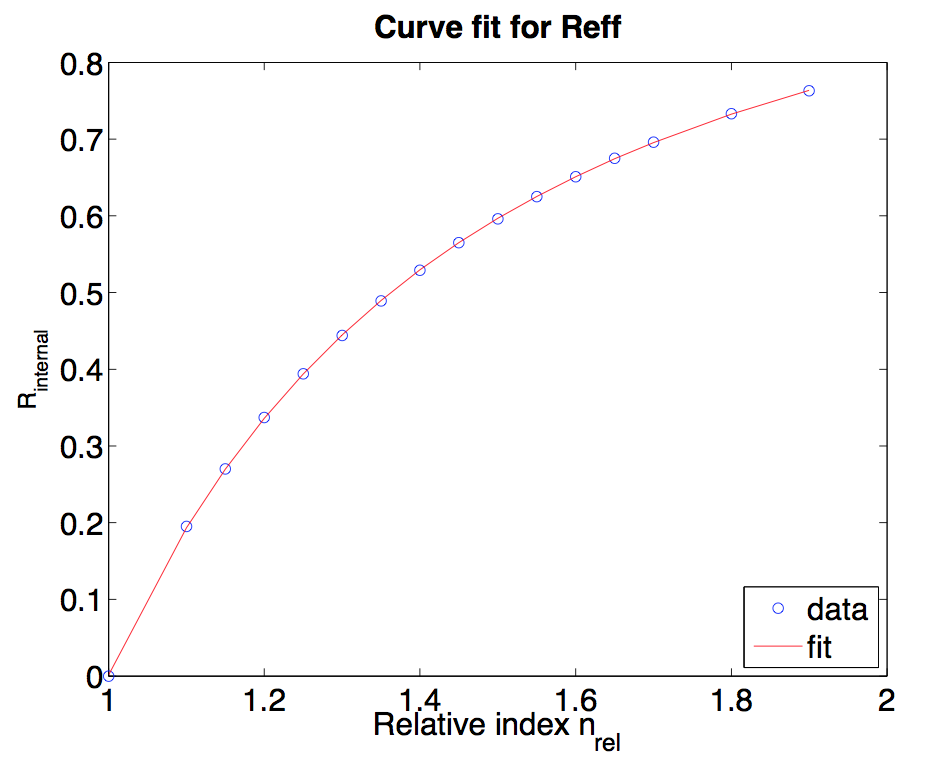
\includegraphics[width=10cm]{./figures/2_Theory/ReflectanceCurveFit.png}
\label{ReflectanceCurveFit}
\caption{A plot showing the tabulated data taken by Orchard fitted with the power series given by Egan.} 
\end{figure}